\chapter{散乱角度}\label{cha:angle}
\section{光生成反応の散乱角度}
図のように$\mu$,中間状態$\gamma^*N$系の散乱角$\theta, \phi$を定義する。\ref{fig:angle1}
\begin{figure}[H]
    \centering
    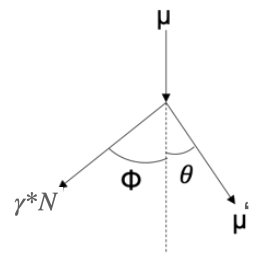
\includegraphics[height=5cm]{img/angle_diagram.png}
    \caption{散乱角$\theta, \phi$の定義}
    \label{fig:angle1}
\end{figure}

\subsection{$\theta$の考察}
下図のような運動学変数を考える。\ref{fig:angle2}
\begin{figure}[H]
    \centering
    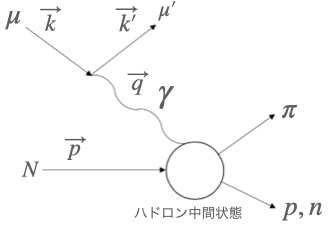
\includegraphics[height=5cm]{img/diagram_3momentum.png}
    \caption{運動学変数の定義}
    \label{fig:angle2}
\end{figure}

各値に対して以下のような定義を行う。
\begin{equation}
    \vec{k} = (E_\mu , p_\mu,0)
\end{equation}
\begin{equation}
    \vec{k'} = (E'_\mu, p'_\mu cos\theta, p'_\mu sin\theta)
\end{equation}
\begin{equation}
    \vec{p} = (m_N, 0, 0)
\end{equation}
\begin{equation}
    \vec{q} = k-k'=(E_\mu - E'_\mu, p_\mu-p'_\mu cos\theta, -p'_\mu sin\theta)
\end{equation}

また、$Q^2$は$\vec{q}$を用いることにより、以下のように表せる。

\begin{equation}
    Q^2 = -q^2 = 2E_\mu E'_\mu -2m^2_\mu-2p_\mu p'_\mu cos\theta
\end{equation}

これを$\theta$について解く。
$E'_\mu = E_\mu(1-y), p'_\mu = \sqrt{E'^2_\mu - m^2_\mu}$
を用いて$E'_\mu, p'_\mu$を消去すると、

\begin{eqnarray}
    \theta & = &\arccos{(\dfrac {2E_\mu E'_\mu -2m^2_\mu-Q^2}{2p_\mu p'_\mu})} \\
    & = & \arccos{(\dfrac{-Q^2-2m^2_\mu+2E^2_\mu(1-y)}{2\sqrt{E^2_\mu-p^2_\mu}\sqrt{E^2_\mu(1-y)^2-m^2_\mu} } )}
\end{eqnarray}

この$\theta$は下図のようになる。\ref{fig:angle3}

\begin{figure}[H]
    \centering
    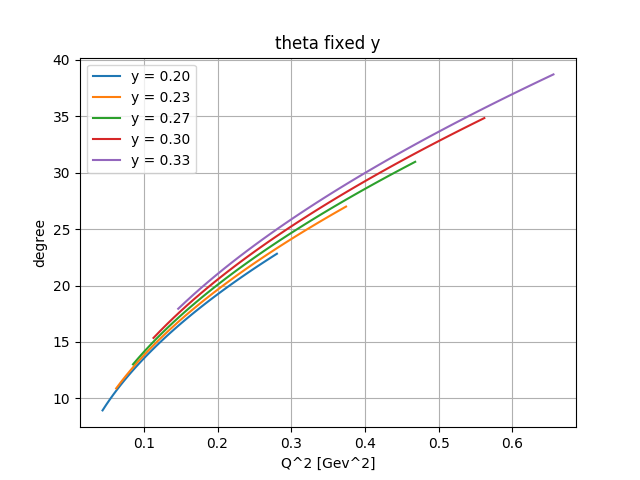
\includegraphics[height=5cm]{img/theta_degree_y_fixed.png}
    \caption{$\mu$の散乱角$\theta$の$Q^2$依存性}
    \label{fig:angle3}
\end{figure}

$\theta$はyが小さくなると小さくなる。また$Q^2$が小さくなると小さくなる。

$\theta$は$\theta=[10^\circ,40^\circ]$の範囲であることがわかる。


\subsection{$\phi$の考察}
\begin{equation}
    \vec{p_\mu} \cdot \vec{p_W} = |p_\mu| |p_W| \cos\phi
\end{equation}
から
\begin{equation}
    \phi = \arccos{(\dfrac{yE^2_\mu + \dfrac{Q^2}{2}} {\sqrt{(E^2_\mu - m^2_\mu)(y^2E^2_\mu+Q^2)}} ) }
\end{equation}
$\phi$は下図のようになる。

\begin{figure}[H]
    \centering
    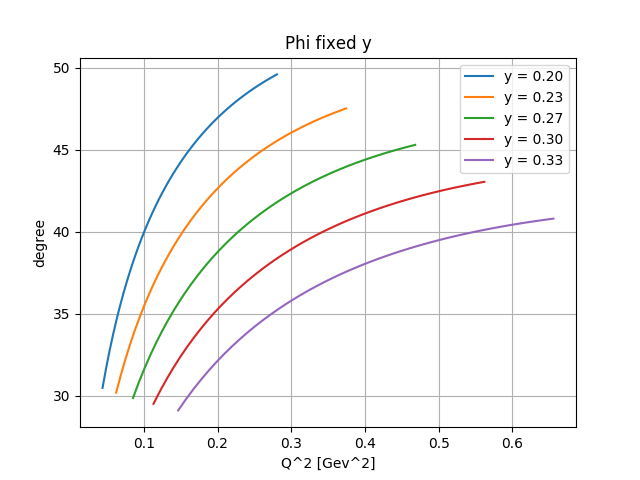
\includegraphics[width=8cm]{img/Phi_degree_fixed_y.png}
    \caption{中間状態の散乱角$\phi$の$Q^2$依存性}
    \label{fig:angle4}
\end{figure}

中間状態の散乱角$\phi$はyが小さくなると大きくなる。また、$Q^2$が小さくなると小さくなる。
$\phi$は$\phi = [30^\circ, 50^\circ]$ の範囲にあることがわかる。

\section{\texorpdfstring{$\gamma N$の崩壊で生成される$\pi, p$について}{LG}}
\subsection{静止した$\gamma N$から生成される$\pi,p$の運動量とエネルギー}\ref{fig:angle5}
\begin{figure}[H]
    \centering
    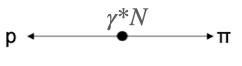
\includegraphics[width=10cm]{img/rest_middle_situation.png}
    \caption{静止した$\gamma N$から生成される$\pi,p$}
    \label{fig:angle5}
\end{figure}
$m_W = 1.08$GeV, $E_\mu = 1.5$GeVを仮定する。
この仮定から$y = 0.2$で$Q^2 \approx 0.28 GeV^2$となる。
それぞれの粒子が持つエネルギーの表式は以下のようになる。
\begin{equation}
    E_\pi = \dfrac{E_W ^2 + m_\pi ^2 - m_p ^2}{2E_W}
\end{equation}

\begin{equation}
    E_p = \dfrac{E_W ^2 + m_p ^2 - m_\pi ^2}{2E_W}
\end{equation}
$E_W = 1.15$GeV, $m_p = 0.938$GeV, $m_\pi = 0.138GeV$として代入すると、
$E_π = 200.7 MeV , E_p = 949.0 MeV , p_π = p_p = 145.8 MeV$となる。


\subsection{ブーストされた$\gamma N$から生成される$\pi,p$の運動量とエネルギー}
\begin{figure}[H]
    \centering
    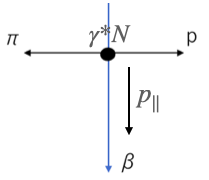
\includegraphics[height=3cm]{img/boost_middle_situation.png}
    \caption{ブーストされた$\gamma N$から生成される$\pi,p$}
    \label{fig:angle6}
\end{figure}

ローレンツ変換を用いて計算する。
\begin{equation}
    \left(\begin{array}{c}
        E^* \\
        p^*_\parallel
    \end{array}\right)
    =\left(\begin{array}{cc}
        \gamma_f \ \ -\gamma_f \beta_f \\
        -\gamma_f \beta _f \ \  \gamma_f
    \end{array}\right)
    \left(\begin{array}{c}
        E \\
        p_\parallel
    \end{array}\right)
\end{equation}

ここで
\begin{eqnarray}
    \beta = \dfrac{p_W}{E_W} = \dfrac{p_\gamma + p_p}{E_\gamma + E_p} = 0.24
\end{eqnarray}

\begin{equation}
    \gamma = 1.03
\end{equation}

となる。
このことから中間状態はあまりブーストされないことがわかる。

\section{\texorpdfstring{ブーストされた$\gamma N$から生成される$\pi$の散乱角}{LG}}
\begin{figure}[H]
    \centering
    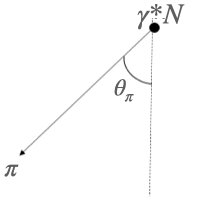
\includegraphics[height=5cm]{img/theta_pi.png}
    \caption{$\pi$の散乱角}
    \label{fig:angle7}
\end{figure}
aa
\begin{figure}[H]
    \centering
    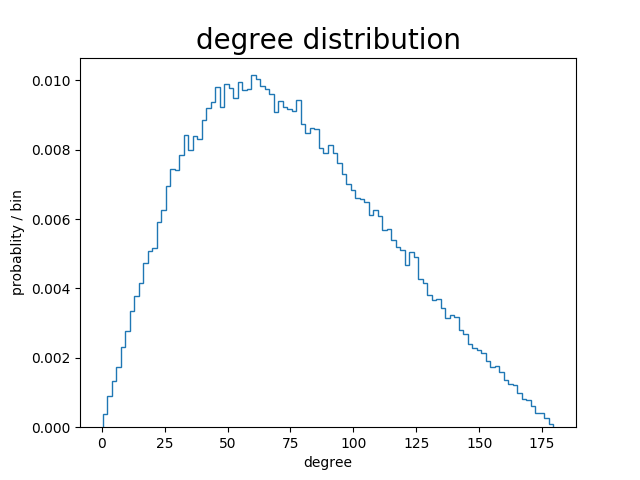
\includegraphics[height=5cm]{img/degree_distribution.png}
    \caption{$\pi$の角度分布}
    \label{fig:angle8}
\end{figure}